%%%%%%%%%%%%%%%%%%%%%%%%%%%%%%%%%%%%%%%%%
% Lachaise Assignment
% LaTeX Template
% Version 1.0 (26/6/2018)
%
% This template originates from:
% http://www.LaTeXTemplates.com
%
% Authors:
% Marion Lachaise & François Févotte
% Vel (vel@LaTeXTemplates.com)
%
% License:
% CC BY-NC-SA 3.0 (http://creativecommons.org/licenses/by-nc-sa/3.0/)
% 
%%%%%%%%%%%%%%%%%%%%%%%%%%%%%%%%%%%%%%%%%

%----------------------------------------------------------------------------------------
%	PACKAGES AND OTHER DOCUMENT CONFIGURATIONS
%----------------------------------------------------------------------------------------

\documentclass{article}

\usepackage{comment}
\usepackage{hyperref}

%%%%%%%%%%%%%%%%%%%%%%%%%%%%%%%%%%%%%%%%%
% Lachaise Assignment
% Structure Specification File
% Version 1.0 (26/6/2018)
%
% This template originates from:
% http://www.LaTeXTemplates.com
%
% Authors:
% Marion Lachaise & François Févotte
% Vel (vel@LaTeXTemplates.com)
%
% License:
% CC BY-NC-SA 3.0 (http://creativecommons.org/licenses/by-nc-sa/3.0/)
% 
%%%%%%%%%%%%%%%%%%%%%%%%%%%%%%%%%%%%%%%%%

%----------------------------------------------------------------------------------------
%	PACKAGES AND OTHER DOCUMENT CONFIGURATIONS
%----------------------------------------------------------------------------------------

\usepackage{amsmath,amsfonts,stmaryrd,amssymb} % Math packages

\usepackage{enumerate} % Custom item numbers for enumerations

\usepackage[ruled]{algorithm2e} % Algorithms

\usepackage[framemethod=tikz]{mdframed} % Allows defining custom boxed/framed environments

\usepackage{listings} % File listings, with syntax highlighting
\lstset{
	basicstyle=\ttfamily, % Typeset listings in monospace font
}

%----------------------------------------------------------------------------------------
%	DOCUMENT MARGINS
%----------------------------------------------------------------------------------------

\usepackage{geometry} % Required for adjusting page dimensions and margins

\geometry{
	paper=a4paper, % Paper size, change to letterpaper for US letter size
	top=2.5cm, % Top margin
	bottom=3cm, % Bottom margin
	left=2.5cm, % Left margin
	right=2.5cm, % Right margin
	headheight=14pt, % Header height
	footskip=1.5cm, % Space from the bottom margin to the baseline of the footer
	headsep=1.2cm, % Space from the top margin to the baseline of the header
	%showframe, % Uncomment to show how the type block is set on the page
}

%----------------------------------------------------------------------------------------
%	FONTS
%----------------------------------------------------------------------------------------

\usepackage[utf8]{inputenc} % Required for inputting international characters
\usepackage[T1]{fontenc} % Output font encoding for international characters

\usepackage{XCharter} % Use the XCharter fonts

%----------------------------------------------------------------------------------------
%	COMMAND LINE ENVIRONMENT
%----------------------------------------------------------------------------------------

% Usage:
% \begin{commandline}
%	\begin{verbatim}
%		$ ls
%		
%		Applications	Desktop	...
%	\end{verbatim}
% \end{commandline}

\mdfdefinestyle{commandline}{
	leftmargin=10pt,
	rightmargin=10pt,
	innerleftmargin=15pt,
	middlelinecolor=black!50!white,
	middlelinewidth=2pt,
	frametitlerule=false,
	backgroundcolor=black!5!white,
	frametitle={Command Line},
	frametitlefont={\normalfont\sffamily\color{white}\hspace{-1em}},
	frametitlebackgroundcolor=black!50!white,
	nobreak,
}

% Define a custom environment for command-line snapshots
\newenvironment{commandline}{
	\medskip
	\begin{mdframed}[style=commandline]
}{
	\end{mdframed}
	\medskip
}

%----------------------------------------------------------------------------------------
%	FILE CONTENTS ENVIRONMENT
%----------------------------------------------------------------------------------------

% Usage:
% \begin{file}[optional filename, defaults to "File"]
%	File contents, for example, with a listings environment
% \end{file}

\mdfdefinestyle{file}{
	innertopmargin=1.6\baselineskip,
	innerbottommargin=0.8\baselineskip,
	topline=false, bottomline=false,
	leftline=false, rightline=false,
	leftmargin=2cm,
	rightmargin=2cm,
	singleextra={%
		\draw[fill=black!10!white](P)++(0,-1.2em)rectangle(P-|O);
		\node[anchor=north west]
		at(P-|O){\ttfamily\mdfilename};
		%
		\def\l{3em}
		\draw(O-|P)++(-\l,0)--++(\l,\l)--(P)--(P-|O)--(O)--cycle;
		\draw(O-|P)++(-\l,0)--++(0,\l)--++(\l,0);
	},
	nobreak,
}

% Define a custom environment for file contents
\newenvironment{file}[1][File]{ % Set the default filename to "File"
	\medskip
	\newcommand{\mdfilename}{#1}
	\begin{mdframed}[style=file]
}{
	\end{mdframed}
	\medskip
}

%----------------------------------------------------------------------------------------
%	NUMBERED QUESTIONS ENVIRONMENT
%----------------------------------------------------------------------------------------

% Usage:
% \begin{question}[optional title]
%	Question contents
% \end{question}

\mdfdefinestyle{question}{
	innertopmargin=1.2\baselineskip,
	innerbottommargin=0.8\baselineskip,
	roundcorner=5pt,
	nobreak,
	singleextra={%
		\draw(P-|O)node[xshift=1em,anchor=west,fill=white,draw,rounded corners=5pt]{%
		Question \theQuestion\questionTitle};
	},
}

\newcounter{Question} % Stores the current question number that gets iterated with each new question

% Define a custom environment for numbered questions
\newenvironment{question}[1][\unskip]{
	\bigskip
	\stepcounter{Question}
	\newcommand{\questionTitle}{~#1}
	\begin{mdframed}[style=question]
}{
	\end{mdframed}
	\medskip
}

%----------------------------------------------------------------------------------------
%	WARNING TEXT ENVIRONMENT
%----------------------------------------------------------------------------------------

% Usage:
% \begin{warn}[optional title, defaults to "Warning:"]
%	Contents
% \end{warn}

\mdfdefinestyle{warning}{
	topline=false, bottomline=false,
	leftline=false, rightline=false,
	nobreak,
	singleextra={%
		\draw(P-|O)++(-0.5em,0)node(tmp1){};
		\draw(P-|O)++(0.5em,0)node(tmp2){};
		\fill[black,rotate around={45:(P-|O)}](tmp1)rectangle(tmp2);
		\node at(P-|O){\color{white}\scriptsize\bf !};
		\draw[very thick](P-|O)++(0,-1em)--(O);%--(O-|P);
	}
}

% Define a custom environment for warning text
\newenvironment{warn}[1][Warning:]{ % Set the default warning to "Warning:"
	\medskip
	\begin{mdframed}[style=warning]
		\noindent{\textbf{#1}}
}{
	\end{mdframed}
}

%----------------------------------------------------------------------------------------
%	INFORMATION ENVIRONMENT
%----------------------------------------------------------------------------------------

% Usage:
% \begin{info}[optional title, defaults to "Info:"]
% 	contents
% 	\end{info}

\mdfdefinestyle{info}{%
	topline=false, bottomline=false,
	leftline=false, rightline=false,
	nobreak,
	singleextra={%
		\fill[black](P-|O)circle[radius=0.4em];
		\node at(P-|O){\color{white}\scriptsize\bf i};
		\draw[very thick](P-|O)++(0,-0.8em)--(O);%--(O-|P);
	}
}

% Define a custom environment for information
\newenvironment{info}[1][Info:]{ % Set the default title to "Info:"
	\medskip
	\begin{mdframed}[style=info]
		\noindent{\textbf{#1}}
}{
	\end{mdframed}
}
 % Include the file specifying the document structure and custom commands

%----------------------------------------------------------------------------------------
%	ASSIGNMENT INFORMATION
%----------------------------------------------------------------------------------------

\title{ CRYPTR: Secure File Sharing \\over the World Wide Web} % Title of the assignment

%\author{Yukiko Amagi\\ \texttt{y.amagi@inabauniversity.jp}} % Author name and email address

\date{} % University, school and/or department name(s) and a date

%----------------------------------------------------------------------------------------

\begin{document}

\maketitle % Print the title


\section*{Introduction}
Securely sharing information over a public network has always been a problem. Most people who use the internet to send files and messages typically don't want outsiders to be able to hijack their messages and steal any personal information such as names, addresses, credit card information. 

SSL/TLS protocols can used to set up secure network connections and securely transfer information over the internet. The issue here is that this requires both parties at each end of the network to be online for the whole duration of the message transmission. This is okay for people who are online all the time, but most people aren't. In the most common case, in order to pass messages and files in an asynchronous manner, people typically use online services such as email, Facebook, Google Drive, or Dropbox. In this case, users upload and download information to the hosting service over a secure network connection and trust that their information is secure on the services' databases. 

 In recent times, it has been shown that many of these online services have been found to be insecure, resulting in personal user files and messages leaked. To combat this, these services have taken extra precautions such as encrypting files internally in order to reassure their users that their information is safe. Despite all these efforts, more external attacks, such as social engineering to steal usernames and passwords, can still be used to bypass these internal security mechanisms.
 
The main problem at hand is, "How can you share a file and get it from point A to point B ensuring the file can be only be read at Point B?". To ensure the utmost amount of security over the untrusted internet, we would have to ensure any files or messages can not be decrypted and read until it reaches it destination. In this assignment we'll play around with what we know about modern cryptography and implement our own way to share files over the untrusted internet, allowing us share files and messages on any service we want by hiding our information in plain sight.

\section*{The problem}
\begin{center}
I want to share a file with friends securely over the untrusted internet.\\ I want to make sure only my friends can see it on their end and no one else.
\end{center}

\subsection*{Solution \#1: Via Secure Connection With SSL/TLS}
If I want to sent a file over the internet, I can simply use SSL/TLS protocols to create a secure connection with my friend. SSL/TLS would automatically use asymmetric key cryptography to generate a temporary shared secret that will be used to encrypt my parts of my file and send it over my network connection to my friend. Due to the use of public-key cryptography, the secret key was agreed upon in such a way  where only me and my friend knows, ensuring that my file encrypted with the secret key is safe.

\begin{figure}[!htb]
        \center{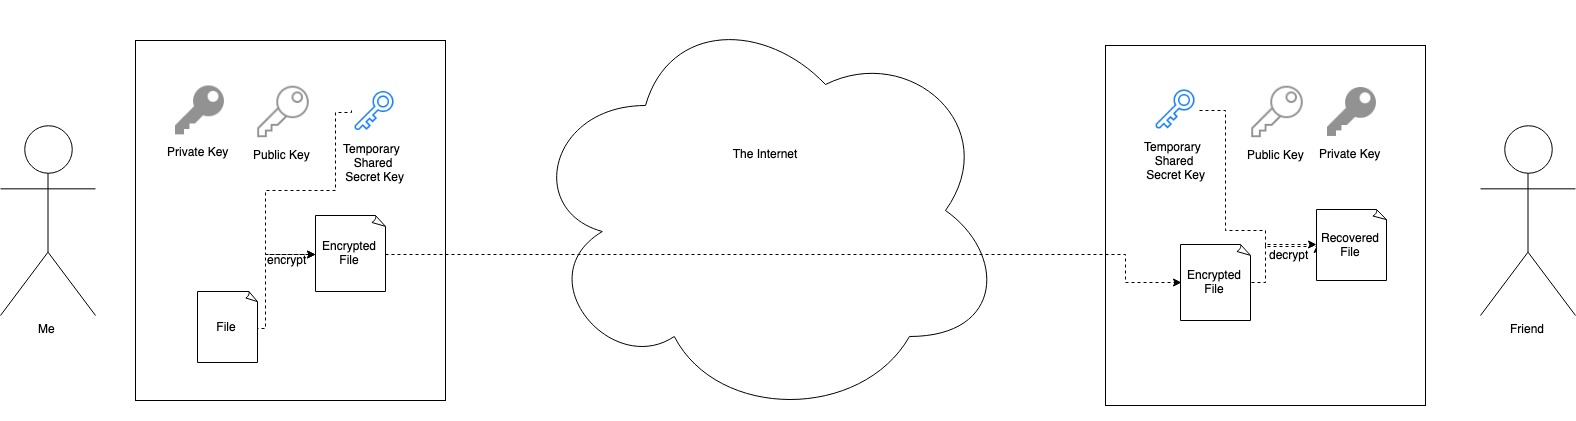
\includegraphics[width=\textwidth]
        {figures/ssltls}}
        \caption{Sending a file via secure connection}
      \end{figure}

\-\\\textbf{The Issue:}
The main issue with this is that both me and my friend have to be connected to the internet at the same time in order to open a network connection to carry out the SSL/TLS protocol. We then both have to stay online until the whole file is sent over. What if both of use are rarely online simultanously? Can we somehow transmit the file in an asynchronous way?

\subsection*{Solution \#2: Via Online Host with Public-Key Cryptography}
In order to share my file with my friend asynchronously I can simply host the file online using a service such as email, Facebook, Google Drive, Dropbox, etc. The issue is that I don't trust services like Facebook or email. I only trust my friend. Because of this, I want to ensure my file is secure even before uploading it. This would require for my friend to upload their public key for me to download. I would then download his public key, encrypt my file, and upload the encrypted file. My friend can then download it and decrypt the file using their private key. Since I used my friend's public key to encrypt my file, I know the encrypted file can only be decrypted by my friend who has the corresponding private key.

\begin{figure}[!htb]
        \center{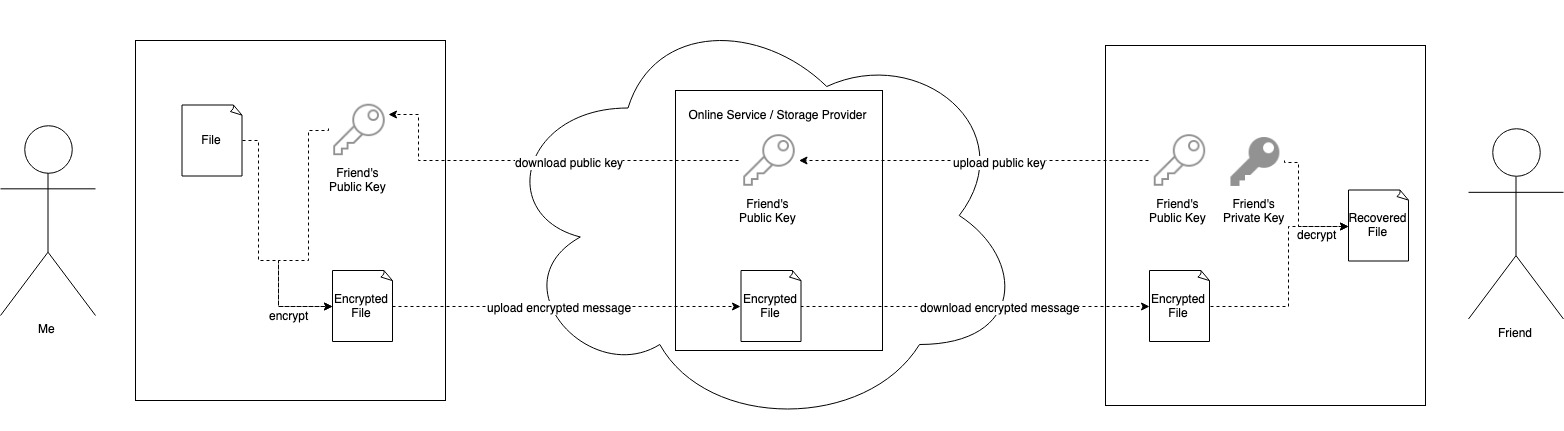
\includegraphics[width=\textwidth]
        {figures/privpubkey}}
        \caption{Sharing a file via online host and public-key cryptography}
\end{figure}


\-\\\ \textbf{The issues:}
\begin{enumerate}
\item I am limited with the file size I can encrypt with a public key. The maximum file size I can encrypt is only as large as the public key size. The typical and recommended key size is 2048 bits, which means I can only encrypt a file up to 256 bytes. What if I want to share files larger than 256 bytes?
\item Even if it were possible to encrypt a file of any size with a public key, because public-key cryptography is asymmetric, only my friend would be able to decrypt my encrypted file. Even though this is what I wanted, this means I would have to re-encrypt the original file and re-upload the resulting encrypted file for each friend I want to share my file with. This would take more time if my file was sufficiently large.
\end{enumerate}


\subsection*{Solution \#3: Via Online Host with Symmetric Key Cryptography}
To be flexible with file size, I can use symmetric key cryptography combined with a block cipher to encrypt a file of any size. In this case, I would generate a secret key, use a block cipher to encrypt my file, then upload my file and key. My friends can then download the encrypted file along with the secret key and use them to recover my original file. In the end, by using a symmetric key I can also avoid having to re-encrypt my file every time I want to share it with friend. \\


\begin{figure}[!htb]
        \center{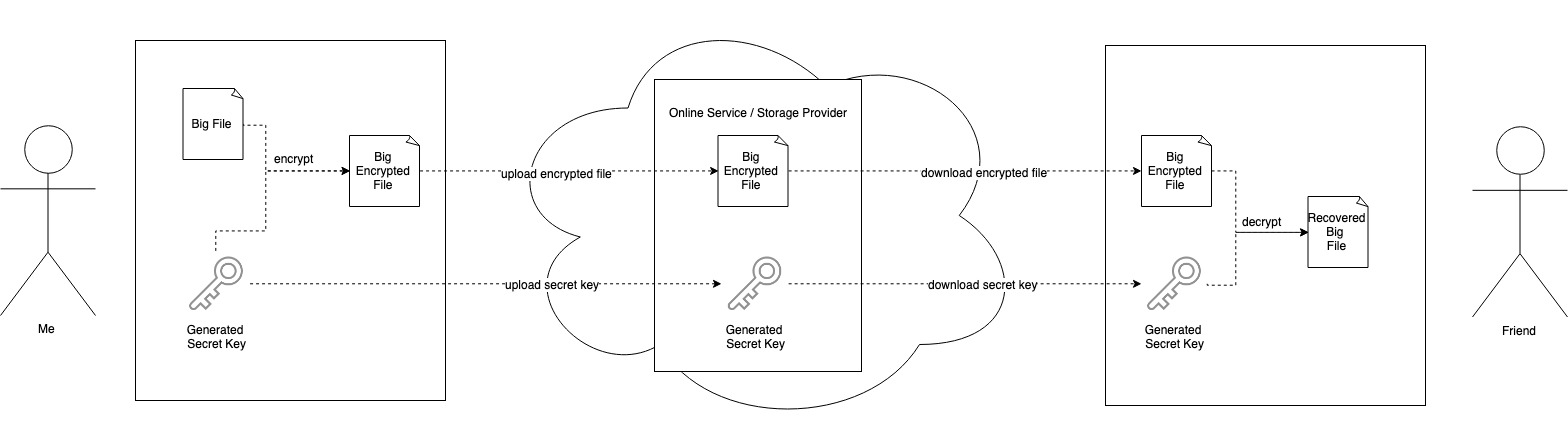
\includegraphics[width=\textwidth]
        {figures/symkey}}
        \caption{Sharing a file via online host and symmetric key cryptography}
\end{figure}


\noindent \textbf{The issue:}\\
With this approach, the secret key is not secure. If the service I was using to host the file was public or hacked, anyone who could access files could download the encrypted file, download the secret key, and recover my original file. How can I securely share the secret key I used to encrypt my file with my friend?


\subsection*{Final Solution: Via Online Host with Symmetric and Public-Key Cryptography}
I can carry out something similar to solution \#3 but instead of sharing the secret key insecurely, I can use public-key cryptography to securely get the secret key to my friend in a similar fashion to solution \#2. Sharing a file would thus be the following process: (1) I would generate a secret key to encrypt my file and upload it. (2) I can then download my friend's public key and use it to encrypt the secret key. (3) I would then upload the encrypted secret key. (4) My friend can then download the encrypted file and encrypted key. (5) Using their private key, my friend can decrypt the secret key which then is used to decrypt the encrypted file. Sharing my file with additional friends would involve steps 2 to 5. 

First, since secret keys for block ciphers are smaller than public/private keys (\textit{128-bit for AES}), I can be sure I can securely encrypt my secret and use this approach to share the secret key in the future. Second, since I only have to encrypt a small key every time I want to share my file with a friend, this is efficient in terms of encryption computation and time it takes to upload. Finally, since my original file is stored on the internet service and I'm securely sharing a secret key that can be used by anyone, I would not have to perform any unnecessary re-encryption and re-uploading of the original file data. 
 
\begin{figure}[!htb]
        \center{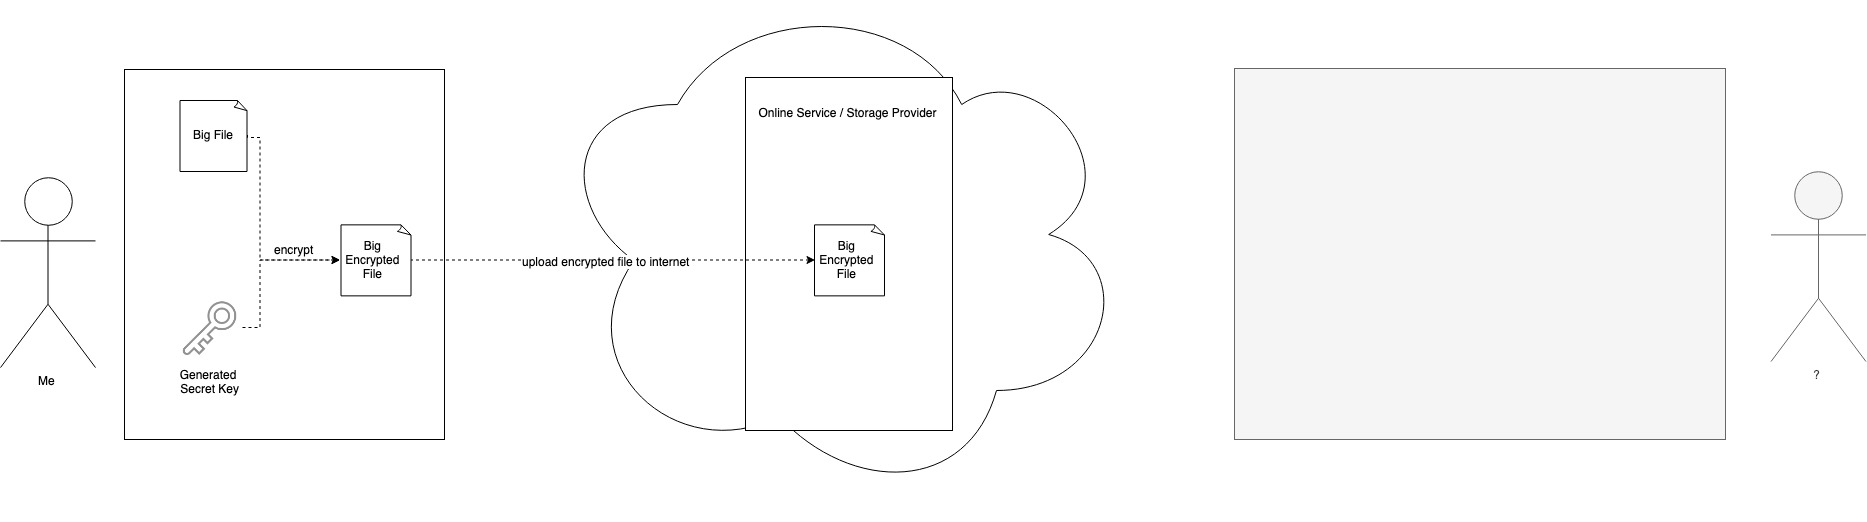
\includegraphics[width=\textwidth]
        {figures/final1}}
        \caption{Uploading an encrypted file using a locally generated secret key, ready for friends to download}
\end{figure}

\begin{figure}[!htb]
        \center{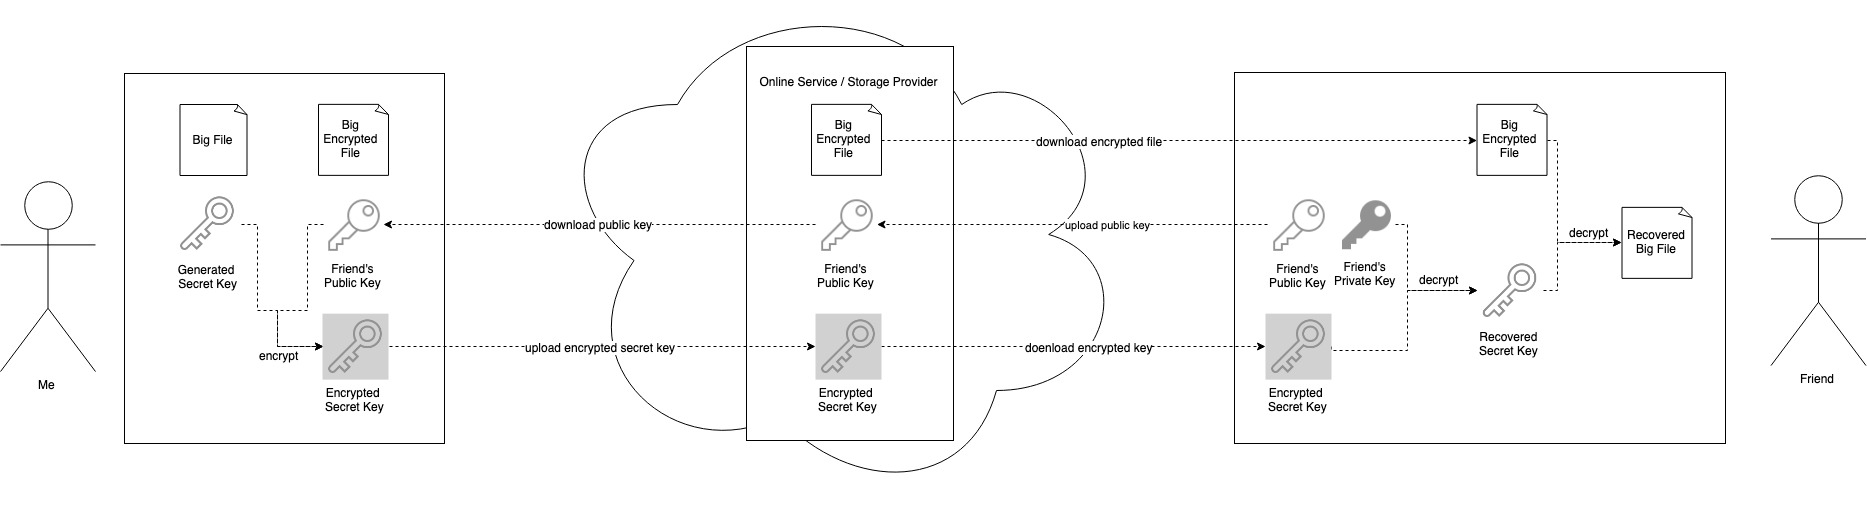
\includegraphics[width=\textwidth]
        {figures/final2}}
        \caption{Sharing secret key using public-key cryptography allowing for friend to decrypt hosted file}
\end{figure}

\-\ \\To sum up, this approach allows us to do the following:
\begin{enumerate}
\item \textbf{Enables us to share a file of an arbitrary size.} Since we're using a block cipher, we can encrypt a file of any size. 
\item \textbf{Enables secure transmission of both file and symmetric key.} Even if the online storage or email server is compromised, no one will be able to decrypt the file without the symmetric key. Although the symmetric key is also stored by some service, no one can decrypt the symmetric key without the receivers private key.
\item \textbf{Enables security with any internet storage provider.} Due to the chain of security supported at the root by public-key cryptography, we can put our encrypted files and encrypted symmetric key anywhere, even on a public forum.
\item \textbf{Enables efficient resource utilization.} Due to the use of both public key and symmetric key encryption, we only need to upload our encrypted file once followed by re-encrypting and re-uploading small secret keys.
\item \textbf{Enables asynchronous distribution.} Whenever I to give someone access to my file, they can download my file at any time and also download the symmetric key at any time. In order to give someone access, I just have to encrypt the symmetric key and share it via dropbox, google drive, email, etc. 
\end{enumerate}



\section*{The Cryptr Program}
In this assignment you will finish implementing a java program called Cryptr that will provide functionalities to carry out the kind of file encryption we need for our newly realized file-sharing protocol.

\-\ \\\noindent The crypt program will support the following functions:
\begin{enumerate}
\item Generating a secret key
\item Encrypting a file using a secret key 
\item Decrypting a file using a secret key
\item Encrypting a secret key using a public key 
\item Decrypting a secret key using a private key
\end{enumerate}


\subsection*{Implementation}
Provided should be a program template called $Cryptr.java$. This template already has a main runner implemented. The program takes in multiple arguments depending on which function wants to carried out. The usage is as follows:

\begin{verbatim}
  Cryptr generatekey <key output file>
  Cryptr encryptfile <file to encrypt> <secret key file> <encrypted output file>
  Cryptr decryptfile <file to decrypt> <secret key file> <decrypted output file>
  Cryptr encryptkey <key to encrypt> <public key to encrypt with> <encrypted key file>
  Cryptr decryptkey <key to decrypt> <private key to decrypt with> <decrypted key file>
\end{verbatim}

\noindent The main method of Cryptr takes the first argument (which specifies the function to do), and calls the respective static method which has the same name of the function specifier but in camel-case. Your job is to use Java's security library ($java.security$) and Java's crypto library ($javax.crypto$) to fill in and implement these static methods so they can carry out their specified functions. As for encryption standards you should follow the recommended security practice of using 2048-bit RSA Keys and at least 128-bit AES keys.
\subsection*{Helpful References}
The following are helpful references to help get you started in understanding how to perform encryption and decryption using Java's security and crypto libraries
\begin{itemize}
\item \textbf{Generating an RSA key pair for Java} \\
Link:  \href{http://codeartisan.blogspot.com/2009/05/public-key-cryptography-in-java.html}{http://codeartisan.blogspot.com/2009/05/public-key-cryptography-in-java.html}\\
\textit{This reference goes over generating RSA key pairs using openssl and converting them to a binary .der file format so that it can be used by a Java program. This also goes how to open and loading the keys into a java program.}
\item \textbf{Public-Key Cryptography in Java}\\ 
Link: \href{https://www.novixys.com/blog/rsa-file-encryption-decryption-java/}{https://www.novixys.com/blog/rsa-file-encryption-decryption-java/}\\
\textit{This reference goes over how to load public and private keys into a Java program as well as use them to encrypt a file}
\item \textbf{Symmetric Key Cryptography in Java (AES)}\\
Link: \href{https://www.novixys.com/blog/java-aes-example/}{https://www.novixys.com/blog/java-aes-example/}\\
\textit{This reference goes over how to generate secret keys, read/write them into a Java program, and use them to perform AES encryption and decryption}
\end{itemize}



\section*{Example Run and Testing}
\subsection*{Compiling the Cryptr program}
We need to compile the program before we use it. 
\begin{commandline}
	\begin{verbatim}
		$ javac Cryptr.java
	\end{verbatim}
\end{commandline}

\subsection*{Generating a file to encrypt}
We'll want to create a sample file to encrypt. We'll just create a simple text file $foo.txt$ that says "This is a text file I want to share".
\begin{commandline}
	\begin{verbatim}
		$ echo "This is a text file I want to share" > foo.txt
	\end{verbatim}
\end{commandline}

\subsection*{Generating a key}
In order to encrypt our file, we will need a secret key stored within a file so that we can encrypt files, This secret key file will not only be used to encrypt a file but the file itself will be encrypted itself to securely share the secret key with whoever we want to be able to decrypt our file. We'll generate a secret key and store it in the file $secret.key$.
\begin{commandline}
	\begin{verbatim}
		$ java Cryptr generatekey secret.key
		Generating secret key and writing it to secret.key
	\end{verbatim}
\end{commandline}

\subsection*{Encrypting File}
Now before we can share our file we have to encrypt it using the secret key. We'll encrypt our file $foo.txt$ with the secret key file we generated $secret.key$ and have the encrypted output be put into a file called $foo.enc$
\begin{commandline}
	\begin{verbatim}
		$ java Cryptr encryptfile foo.txt secret.key foo.enc
		Encrypting foo.txt with key secret.key to foo.enc
	\end{verbatim}
\end{commandline}

\subsection*{Generating Key Pair}
We need to generate a sample RSA key pair to represent the public and private keys of our friend. These need to be converted into the $.der$ format to be used with our Java program. We'll name the private key $private\_key.der$ and the public key $public\_key.der$.
\begin{commandline}
	\begin{verbatim}
		$ openssl genrsa -out private_key.pem 2048
		$ openssl pkcs8 -topk8 -inform PEM -outform DER -in private_key.pem \
		-out private_key.der -nocrypt
		$ openssl rsa -in private_key.pem -pubout -outform DER -out public_key.der
	\end{verbatim}
\end{commandline}


\subsection*{Encrypting the Secret Key}
Now that we have a sample key pair, let's encrypt the secret key file $secret.key$ with the public key $public\_key.der$ and output it to a file called $s.enckey$. 
\begin{commandline}
	\begin{verbatim}
		$ java Cryptr encryptkey secret.key public_key.der s.enckey
		Encrypting key file secrey.key with public key file public_key.der to s.enckey
	\end{verbatim}
\end{commandline}


\subsection*{Decrypting Key and File}
Finally in order to decrypt the file, we should be able to decrypt the encrypted secret key and then use that key to decrypt the encrypted file. First we'll decrypt the encrypted secret key file $s.enkey$ with the private key $private\_key.der$ and put it in a file called $recovered-secret.key$. Then we'll decrypt the encrypted file $foo.enc$ with the recovered secret key $recovered-secret.key$ and put it in a file called $recovered-foo.txt$.
\begin{commandline}
	\begin{verbatim}
		$ java Cryptr decryptkey s.enckey private_key.der recovered-secret.key
		Decrypting key file s.enckey with private key file private_key.der to 
		recovered-secret.key
		$ java Cryptr decryptfile foo.enc recovered-secret.key recovered-foo.txt
		Decrypting foo.enc with key recovered-secret.key to recovered-foo.txt
	\end{verbatim}
\end{commandline}
Printing out the recovered text file using the $cat$ command should show us the contents of our original file. 
\begin{commandline}
	\begin{verbatim}
		$ cat recovered-foo.txt
		This is a text file I want to share
	\end{verbatim}
\end{commandline}

\section*{Grading}
You will not be graded on the output of the program. Your code will be checked to confirm the usage of the proper libraries. It will be compiled and called to perform the different functions. The resulting files will be examined and then we will check for whether or not the original file can be recovered similar to the process shown in the example run. 

\section*{Submissions}
To submit your assignment, simply submit your $Cryptr.java$ file directly to sakai as is. Do not compress the java file, as it will be easier for us to grade. \textbf{If you worked on the code within an IDE which required a package structure, please remove the package statement prior to submission to allow for us to compile the Java program without a package structure.}

\section*{Additional Tips and Tricks}

\begin{info}[Print Statements Galore:]
You will not be graded on the output of the program, simply just the actual contents of the files your program makes and whether or not the original file can be recovered like shown in the example run. Because of this, feel free to make any additional print statements you see fit. 
\end{info}

\begin{comment}
\begin{info}[Throw 'Em All Away:] 
Using more advanced libraries, there will be many exceptions that these methods can potentially throw. You are \textbf{not required} to catch these exceptions and error out of the program softly. If your implementation is correct, no exceptions should be thrown, so if you don't want to handle them explicitly it is acceptable for this assignment to throw them using the $throws$ declaration. It should be noted that this is bad practice. 
\end{info}
\end{comment}

\begin{info}[Remember to Pad:] 
Remember that with block ciphers, padding is needed to ensure data aligns with the cipher being used. For example, we know AES with a 128-bit key encrypts 128-bit blocks (16 bytes) at a time, if you have a 58 byte file and you encrypt the first 3 blocks (48 bytes), the cipher will not be able to continue and encrypt those last 10 bytes since its less than a block size. An exception \textbf{WILL} be thrown. In this case, an extra 6 bytes should be added to allow for the cipher to encrypt the last 10 bytes within a 16 byte block size. Consult references to get an idea of how you can pad your data.
\end{info}

\begin{info}[When in doubt, Google:]
If you have an issue or your program is throwing an error that you don't know how to fix, Google It. Someone, somewhere, probably faced the same issue at some point.
\end{info}

\section*{Frequently Asked Questions}
\begin{itemize}
\item \textbf{Is Java 8 fine?} Yes.
\item \textbf{Can I use lambdas?} Yes, Java 8 is fine as previously mentioned.
\item \textbf{Can I use any other non-standard Java libraries?} You shouldn't have to. No.
\item \textbf{Can I do this assignment in Python/Go/JS/Ruby/PHP/C++/C/Scheme?} I'm Sorry. Java.
\end{itemize}

\section*{Additional Questions}
If you have any questions about the assignment or are having any issues, email me at David.Domingo@rutgers.edu






\end{document}
